\documentclass{article}
\usepackage{tikz}
\usetikzlibrary{matrix}
\begin{document}
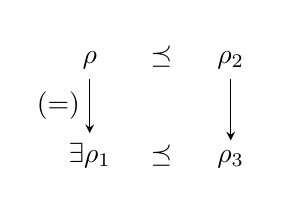
\begin{tikzpicture}
  \matrix (m) [matrix of math nodes,row sep=2em,column sep=0.5em,minimum width=2em]
  {
     \rho &\preceq& \rho_2 \\
    \exists \rho_1 &\preceq & \rho_3 \\};
  \path[-stealth]
    (m-1-1) edge node [left] {($=$)} (m-2-1)
    (m-1-3) edge node [left] {} (m-2-3);
\end{tikzpicture}


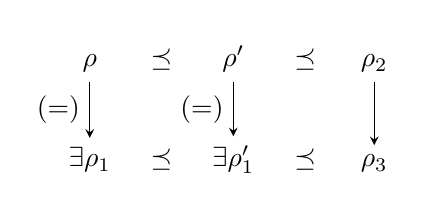
\begin{tikzpicture}
  \matrix (m) [matrix of math nodes,row sep=2em,column sep=0.5em,minimum width=2em]
  {
    \rho &\preceq& \rho' &\preceq& \rho_2 \\
    \exists\rho_1 &\preceq&\exists \rho'_1 &\preceq & \rho_3 \\};
  \path[-stealth]
    (m-1-1) edge node [left] {($=$)} (m-2-1)
    (m-1-3) edge node [left] {($=$)} (m-2-3)
    (m-1-5) edge node [left] {} (m-2-5);

\end{tikzpicture}
\end{document}